\chapter{Modelli mentali}\index{modelli mentali}
\section{Metodi di ragionamento}
La capacità di compiere deduzioni è considerata la caratteristica essenziale che definisce la razionalità dell’individuo, a sua volta vista come la funzione definitoria dell’uomo rispetto a tutto cioè che non è uomo.

Nell’approccio dei \emph{modelli mentali} il ragionamento non si fonda sull’applicazione di regole logiche di inferenza, ma sulla manipolazione di modelli mentali che rappresentano gli stati di cose specifici su cui si ragiona.

Si distingue principalmente in due tipi di ragionamento, la \emph{deduzione}\index{deduzione} e l’\emph{induzione}\index{induzione}. La deduzione è un modo di procedere dal generale verso il particolare, che garantisce la validità delle conclusioni ottenute. Prendiamo l’esempio

\syllogC{Tutti gli uomini sono mortali}{Socrate è un uomo}{Quindi, Socrate è mortale}
	
La validità della conclusione non implica la verità della conclusione stessa. Questa dipende dal fatto che le premesse siano vere, e quindi impone una verifica sulle cose affermate che non ha niente a che fare con la deduzione vera e propria. Se per esempio una sola premessa è falsa, la conclusione diventa falsa, ma la forma deduttiva conserva la sua validità:

\syllogC{Tutti gli uomini hanno due mani}{Capitan Uncino è un uomo}{Quindi, Capitan Uncino ha due mani}

L’induzione è il modo di procedere inverso, che va dal particolare al generale. L’induzione non si fonda su leggi generali e non può mai garantire la validità delle conclusioni. Potremmo affermare che la conoscenza umana sia sempre di tipo induttivo, dato che non abbiamo modo di accedere a verità ultime, ma incontriamo sempre fatti particolari.

L’obiettivo del sistema inferenziale non è produrre tutte le possibili conclusioni lecitamente derivabili da un insieme di premesse, ma derivare solo quelle \emph{interessanti}. Nessun sistema deduttivo accresce la conoscenza, perché ogni deduzione è sempre tautologica; in altri termini, tutte le conclusioni valide erano implicitamente presenti già nelle premesse, sono solo state evidenziate nella conclusione. Ciò nonostante, il rendere esplicita una parte della conoscenza implicita può essere altamente informativo, perché nessun essere umano è in grado di cogliere immediatamente tutte le possibili conclusioni data una serie di premesse. Si tratta di distinguere tra conclusioni solo valide e conclusioni sia valide che interessanti.

Secondo l’ipotesi modellistica, alla base del ragionamento vi è un’attività di manipolazione di modelli di situazioni specifiche, piuttosto che l’applicazione di regole di inferenza su strutture simboliche astratte. L’ipotesi dell’uso di modelli porta a considerare il ragionamento come un’attività fortemente dipendente dal dominio di applicazione; studiare il ragionamento implica quindi la ricerca di uno spettro di domini significativi e l’individuazione delle classi di modelli che li caratterizzano.

\section{Deduzione tramite modelli mentali}\index{modelli mentali}
Il contributo alla psicologia e alla scienza cognitiva per cui è più noto Philip Johnson-Laird\index{Johnson-Laird, Philip}\footnote{Philip Johnson-Laird (Leeds, 12 ottobre 1936) è uno psicologo britannico. Si è occupato soprattutto di psicologia del linguaggio e del ragionamento.} è la teoria dei modelli mentali. Concepita inizialmente come una teoria del ragionamento sillogistico (cioè dei processi mentali eseguiti da un soggetto che cerca di trarre una conclusione dalle premesse di un sillogismo), la teoria è stata estesa ad altri tipi di ragionamento e alla comprensione del linguaggio naturale. Secondo Johnson-Laird, un sillogismo è valutato costruendo un modello mentale integrato delle premesse e visualizzando la relazione tra i termini estremi che figurano nel modello integrato. L'integrazione dei modelli delle premesse può avvenire in più di un modo, ed è verosimile che un sillogismo sia tanto più \emph{difficile} quanto più numerosi sono i modelli integrati costruibili. Questa previsione è infatti confermata dai dati sulle prestazioni di soggetti umani impegnati nella risoluzione di sillogismi.

\begin{figure}[hbt]
  \centering
  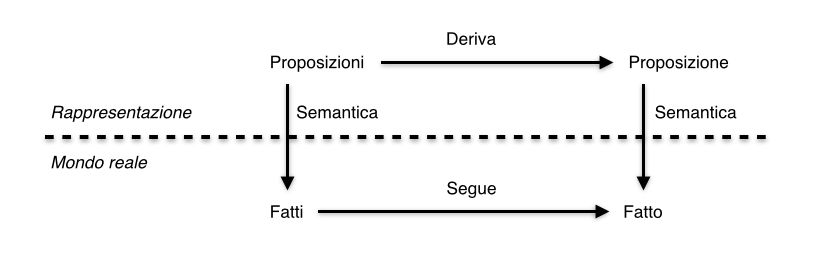
\includegraphics[width=\textwidth]{img/deduzione.png}
  \caption{Schema della deduzione tramite modello mentale}
  \label{fig:modello-mentale}
\end{figure}

Nel 1958 Jean Piaget\index{Piaget, Jean}\footnote{Jean Piaget (Neuchâtel, 9 agosto 1896 – Ginevra, 16 settembre 1980) è stato uno psicologo, biologo, pedagogista e filosofo svizzero.}, all'interno della sua teoria del pensiero e dell’intelligenza, in cui sostiene che i bambini si costruiscono una competenza logica interiorizzando le azioni che compiono e riflettendo su di esse, postula l'esistenza di una logica mentale tale per cui «il ragionamento non è nient'altro che il calcolo proposizionale in quanto tale». Il pensiero dell’adulto quindi ha la forma della logica formale aristotelica, ovvero che il pensiero è naturalmente logico.

Piaget afferma che attorno ai 12 anni si entra nella fase del ragionamento formale, che coinvolge operazioni logiche fatte su pensieri astratti, comunemente chiamato ragionamento ipotetico. Un famoso esempio di studio riguarda un gioco di carte in cui ogni carta ha una lettera su una faccia e un numero sull’altra, come mostrato nella figura \ref{fig:deduzione}; se c’è una vocale da un lato, dall’altro lato c’è un numero pari.

\begin{figure}[hbt]
  \centering
  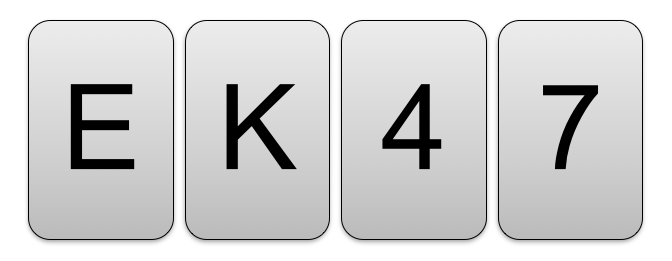
\includegraphics[width=.6\textwidth]{img/ek47.png}
  \caption{Esempio di test sulla deduzione}
  \label{fig:deduzione}
\end{figure}


Il gioco consiste nel dire quali carte è necessario girare per verificare se la regola è vera. Gli errori di contrapposizione e di biimplicazione si verificano nel 60\% dei soggetti.\footnote{La risposta è “E” e “7”. La “E” deve avare un pari dietro, il “7” non deve avere una vocale. Le regole non dicono su cosa deve esserci dietro una consonante come “K” e neanche che il “4” deve avere una vocale dall’altro lato.}

Cambiando però il contenuto delle carte (località/mezzo di trasporto) con l’asserzione “ogni volta che vado a X prendo il treno” le prestazioni migliorano, si verifica solo il 12\% degli errori. La conclusione è che il contenuto aiuta il ragionamento e le inferenze non sono basate solo sulla forma logica.

Simultaneamente alla costruzione del programma logicista nella cognizione, alcuni ricercatori come Wason, nel tentativo di verificare le posizioni di Piaget, trovarono alcuni risultati completamente discordanti. In alcuni esperimenti le persone sorprendentemente si comportano sistematicamente in modo illogico. Questa dissonanza emersa tra il paradigma logicista della scienza cognitiva e questi risultati portarono alla conclusione che le performance illogiche derivassero da fraintendimenti delle premesse o dall’applicazione sbagliata delle regole logice. Mary Henle, psicologa, dichiarò «non ho mai trovato errori che possano in modo non ambiguo essere attribuiti al ragionamento fallace».

\subsection{Falsificazione}
Falsificare un’ipotesi, una legge o una regola, equivale a dimostrarne la falsità mettendo in evidenza almeno un caso che la viola (controesempio): questa operazione viene chiamata “falsificazione” ed è molto usata nell’ambito del ragionamento scientifico.

Nella vita naturale invece tendiamo a costruire regole che grosso modo funzionino, procedendo alla loro verifica, nelle varie situazioni pratiche, più che tentare strategie falsificanti. Ciò porta a difficoltà del pensiero naturale nei ragionamenti nei quali occorre falsificare per raggiungere una conclusione. Ne abbiamo un esempio nel problema delle quattro carte di Wason e nella difficoltà a trarre corrette conclusione nei sillogismi condizionali.

\section{I modelli mentali}
I modelli mentali sono un tipo di struttura dati dinamica in grado di rappresentare, attraverso un formato semi-analogico, vari domini di conoscenza (reali, ipotetici, immaginari). Secondo Johnson-Laird (1989) un modello mentale è caratterizzato dalle seguenti proprietà:

\begin{itemize}
  \item La struttura di un modello corrisponde alla struttura della situazione rappresentata nel modello.
  \item Un modello contiene elementi corrispondenti solo ad entità percepite (perceptible entities) ma, all’occorrenza, può contenere anche elementi corrispondenti a concetti astratti (abstract notions) che dipendono, in modo decisivo, dalle procedure utilizzate per la manipolazione dei modelli. 
  \item È un tipo di rappresentazione mentale che non contiene variabili e che può includere soltanto un numero finito di occorrenze individuali.
  \item Un modello è da considerarsi il risultato finale (output) di cinque procedure generali (START, ADD, COMBINE, VERIFY, USE) e due procedure ricorsive (REVISE, REVISE) operanti nei confronti delle occorrenze contenute nel modello.
\end{itemize}

Prendiamo, per esempio, l’ormai classico caso delle relazioni spaziali. Si consideri la premessa: “Il triangolo è a destra del cerchio.”
\[\bigcirc \bigtriangleup\]

La sua rappresentazione proposizionale è \texttt{rightOf(cicle, triangle)} e i suoi predicati sono distribuiti secondo la sintassi del pensiero. La rappresentazione con un modello mentale invece è isomorfa alla relazione spaziale reale e la forma e le dimensioni possono essere riviste in seguito ad altre premesse.

\subsection{Isomorfismo}\index{isomorfismo}
Un  elemento di divergenza rispetto alle ``strutture ricordate'' è che i modelli mentali sono, per definizione, \emph{isomorfici} a ciò che rappresentano, nel senso che nel modello viene mantenuta ``la stessa struttura di rapporti'' che esiste tra gli elementi del dominio rappresentato (come mostrato nell’esempio precedente). Strutture rappresentazionali come frames, scripts e schemi, inoltre, non descrivono in che modo le parole si riferiscono al mondo. La teoria dei modelli mentali assume, invece, che la comprensione di un enunciato corrisponda ad afferrare le sue condizioni di veritaà.

Compatibilmente con una concezione internista della verità, Johnson-Laird sostiene che il riferimento di un dato enunciato viene individuato dallo stato di cose immaginato che rende vera la situazione descritta dall’enunciato in oggetto: si immagina uno stato di cose (si costruisce un modello mentale dell’enunciato) che corrisponde a “come sarebbe il mondo se l’asserzione venisse considerata vera”.

Lo stato di cose immaginato corrisponde alla sua rappresentazione mentale, mentre il valore di verità dell’asserzione considerata può essere accertato comparando la rappresentazione mentale con lo stato di cose del mondo (percepibile) che essa descrive.

Cosa significa riconoscere che un dato enunciato è vero? Si tratta, crediamo, di effettuare un’immersione (in un senso matematico, darne un’interpretazione relativa) del modello mentale dell’enunciato considerato nel modello percettivo originario.

L’ipotesi che formuliamo si basa sull’accezione matematica del termine immersione. In matematica, infatti, tale termine indica una relazione tra due strutture tali che una delle due contiene all’interno una ``copia'' dell’altra: in questo senso la struttura di un modello percettivo ``contiene'' al suo interno una copia del modello mentale, dato che questo è considerato come la versione schematica del modello percettivo originario.

Se, però, è possibile immergere un modello in un altro, data una certa compatibilità strutturale, in che senso possiamo immergere un enunciato in un modello? Facciamo notare che per Johnson-Laird i modelli percettivi costituiscono l’interfaccia privilegiata con il nostro ambiente sensoriale, sono, cioè, rappresentazioni ``compatte'' del mondo. Senza tale incorporazione, un dato enunciato risulta privo di significato, inaccessibile alla mente.

Si tratterebbe di costruire e recuperare tali rappresentazioni compatte del mondo, internalizzarle (ecco che diventano mentali) e utilizzarle per ragionare e per comprendere un qualsiasi insieme di enunciati. Tale processo consentirebbe alla mente un accesso naturale alla verità, intesa come meta-proprietà di un enunciato che si ``afferra'' solo se è possibile immaginare la struttura percettivo-spaziale di quell’enunciato.

Secondo tale concezione, la verità è una proprietà costitutiva dei modelli, interna, sostanziale (condivisa con la struttura dei nostri corpi, così come dei nostri ambienti di vita). In tal senso, comprendere la verità di un enunciato equivale, cognitivamente, ad ancorare percettivamente l’enunciato. Supponiamo, con Johnson-Laird, che sia così: si potrebbe dire che a parti di modello corrispondono parti di mondo proiettati nel modello. Le proprietà geometriche della struttura del vivente (quindi anche dei nostri corpi) saranno mantenute nei modelli mentali: le caratteristiche topologiche di un oggetto dovranno essere mantenute nel modello di tale oggetto. Un modello mentale di un pallone che ruota nel campo visivo, non avrà la struttura di un toro, per intenderci; se, infatti, diamo a qualcuno il compito di disegnare un albero, con molta probabilità, disegnerà una figura che manterrà il principio di continuità nella rappresentazione (mentale): la persona, pur deformando a piacere la figura, utilizzerà rappresentazioni continue della figura rappresentata. È interessante notare come la continuità sia mantenuta anche nella rappresentazione mimica dell’oggetto che ruota: una mano che ruota, ad esempio, simula una cicloide.

Quando diciamo che un modello mentale (che è una versione più schematica di un’immagine mentale e che può contenere contrassegni simbolici) è \emph{isomorfo} al dominio rappresentato, facciamo alcune ipotesi sul tipo e sul formato di rappresentazioni mentali manipolate.

Geometricamente, tale isomorfismo sarebbe la realizzazione mentale di un’\emph{iniezione}, nel preciso senso matematico, tra i ``punti'' del modello percettivo e i ``punti'' del modello mentale: in una fotografia, per esempio, dobbiamo poter riconoscere un’immagine rappresentata ed è necessario che siano conservate determinati invarianti strutturali. Punti allineati dell’oggetto devono andare in punti allineati della fotografia, le lunghezze e le dimensioni non saranno alterate eccessivamente, non saranno, cioè, tutte rappresentate in un punto di singolarità e dovrà essere conservata la relazione di vicinanza tra punti: nel modello, come nella fotografia, verrà rispettata la struttura topologica del dominio rappresentato.

Tali assunzioni, precisiamolo, riguardano la natura dei modelli concepiti come strutture cognitive astratte: non sappiamo se ad un livello corticale o sub corticale vi sia un rapporto in scala tra mappe neurali o se esista una corrispondenza punto a punto tra ipotetiche mappe corticali in grado di implementare i processi mentali coinvolti nella genesi di un modello mentale.

\section{Inferenza sillogistica}\index{sillogismi}
I sillogismi hanno da sempre costituito il banco di prova preferenziale delle teorie psicologiche sul ragionamento. Di essi si sa tutto, dato che sono stati indagati ininterrottamente per 2400 anni, da Aristotele ad oggi; rappresentano un insieme di 64 problemi diversi, di vari gradi di difficoltà, utilmente collegati fra loro. I sillogismi sono deduzioni basate su due premesse, da cui si deve inferire la conclusione corretta. Le premesse consistono di proposizioni in cui compaiono quantificatori.

Secondo la teoria di Johnson-Laird, tre sono i fattori fondamentali da cui dipendono le prestazioni dei soggetti sperimentali nella risoluzione di un’inferenza sillogistica:

\begin{enumerate}
  \item differente complessità di elaborazione delle premesse legata alla figura delle premesse stesse, in ordine di complessità crescente dalla prima alla quarta;
  \item numero di modelli che è necessario costruire per verificare la validità di una conclusione in ciascun sillogismo: una conclusione è valida solo se si dimostra che è compatibile con tutti i modelli significativamente diversi che si possono costruire;
  \item limitazione delle risorse cognitive, in particolare la diversa capacità della memoria di servizio mostrata dai soggetti.
\end{enumerate}

Nella risoluzione di sillogismi, parallelamente a quanto accade in ogni altra attività di ragionamento, possiamo distinguere tre diversi momenti: costruzione, manipolazione e verifica dei modelli mentali in questione.

\begin{description}
  \item[Costruzione] Nell’inferenza sillogistica, questa fase corrisponde all’interpretazione delle premesse; per ciascuna premessa i soggetti costruiscono un modello mentale che rappresenta lo stato di cose da essa descritta; si avranno così due modelli separati ciascuno costituito da un numero finito di elementi, che rappresentano individui, e relazioni fra individui;
  \item[Integrazione] Questa fase consiste nell’integrare fra loro i modelli separati di ciascuna premessa, formando un unico modello integrato che si può leggere per trovare la conclusione. Nel modello integrato si pongono relazioni fra gli elementi che rappresentano i termini A e C, fra i quali non c’erano nelle premesse relazioni esplicite; in tal modo, il modello integrato rappresenta una conclusione informativa;
  \item[Verifica] In questa fase avviene il tentativo di falsificare la conclusione ottenuta; coerentemente a quanto suggerito da Popper in epistemologia, la verifica della validità di una conclusione si realizza attraverso la ricerca di controesempi. Applicando ricorsivamente la funzione precedente vengono generati modelli integrati alternativi, ciascuno dei quali rappresenta una possibile conclusione; la funzione di verifica confronta ciascuna conclusione ottenuta con lo stato di cose descritto dagli altri modelli integrati. Se una conclusione risulta compatibile con tutti i modelli integrati generati, tale conclusione sarà considerata valida; se, viceversa, tutte le conclusioni sono falsificate da almeno uno dei modelli integrati, allora nessuna conclusione valida risulta possibile.
\end{description}

L’insistenza sul fatto che la teoria dei modelli mentali spiega le inferenze sillogistiche con una precisione impensabile per la teoria della logica mentale è dovuta alla considerazione che se i modelli mentali si dimostrano più efficaci della logica mentale proprio nell’ambito privilegiato da quest’ultima, viene estremamente rinforzata la loro posizione teoretica. Che i modelli mentali siano efficaci in un ambito di ragionamento quotidiano, potrebbe sembrare troppo semplice: che lo siano nell’area del pensiero formale, assume tutt’altro significato. Per quanto riguarda gli aspetti evolutivi, la teoria dei modelli mentali sembra anche qui cominciare a offrire una ricchezza di predizione sconosciuta agli altri approcci, anche se per ora troppo settoriale da permettere di nutrire ambizioni immediate di sostituire le teorie evolutive classiche.